\section{Introduction}
\label{sec:introduction_006}

In \cref{chap:introduction,chap:background}, we have reviewed the motivation and background for uncertainty estimation for independent and non-independent data in ML. In this part, we first focus on uncertainty estimation on independent data (e.g. tabular or images). To this end, we start in this chapter to focus on uncertainty estimation for the well-established classification tasks. Despite the necessity for accurate uncertainty estimation, traditional neural networks for classification tasks cannot distinguish between aleatoric and epistemic uncertainty and show overconfident predictions, even for data that is significantly different from the training data \cite{ensembles} \cite{calibration-network}.

As discussed in \cref{sec:background-models}, multiple uncertainty methods proposed to mitigate this problem. In particular, many methods like ensembles, variational Inference, MC Dropout, MCMC have demonstrated remarkable performance but only describe implicit distributions for predictions which require a costly sampling phase for uncertainty estimation.

% In particular, they should distinguish between \emph{aleatoric} and \emph{epistemic} uncertainty, also called data and knowledge uncertainty \cite{PriorNetworks}, respectively. The aleatoric uncertainty is irreducible from the data, e.g. a fair coin has 50/50 chance for head. The epistemic uncertainty is due to the lack of knowledge about unseen data, e.g. an image of an unknown object or an outlier in the data. 

% Quantifying uncertainty in neural network predictions is key to making Machine Learning reliable. In many sensitive domains, like robotics, financial or medical areas, giving autonomy to AI systems is highly dependent on the trust we can assign to them. In addition, AI systems being aware about their predictions' uncertainty, can adapt to new situations and refrain from taking decisions in unknown or unsafe conditions. Despite this necessity, traditional neural networks show overconfident predictions, even for data that is significantly different from the training data \cite{ensembles} \cite{calibration-network}. 
% In particular, they should distinguish between \emph{aleatoric} and \emph{epistemic} uncertainty, also called data and knowledge uncertainty \cite{PriorNetworks}, respectively. The aleatoric uncertainty is irreducible from the data, e.g. a fair coin has 50/50 chance for head. The epistemic uncertainty is due to the lack of knowledge about unseen data, e.g. an image of an unknown object or an outlier in the data.

\begin{figure}[ht!]
    \centering
    \begin{subfigure}[t]{0.23 \columnwidth}
        \centering
        
\includegraphics[width=0.8 \textwidth]{sections/006_neurips2020/figures/2D_latent_klpn_2.png}
         \caption{Data labels - PriorNet}
         \label{KLPN_visualization_2D}
    \end{subfigure}%
    \begin{subfigure}[t]{0.23\columnwidth}
        \centering
        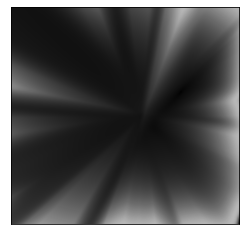
\includegraphics[width=0.8 \textwidth]{sections/006_neurips2020/figures/2D_latent_klpn_1.png}
        \caption{Uncertainty - PriorNet}
        \label{KLPN_visualization_unc}
    \end{subfigure}%
    \begin{subfigure}[t]{0.23 \columnwidth}
        \centering
        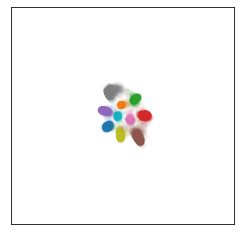
\includegraphics[width=0.8 \textwidth]{sections/006_neurips2020/figures/2D_latent_ours_bn_2.png}
         \caption{Data labels - \PostNetacro}
         \label{ours_visualization_2D}
    \end{subfigure}%
    \begin{subfigure}[t]{0.23\columnwidth}
        \centering
        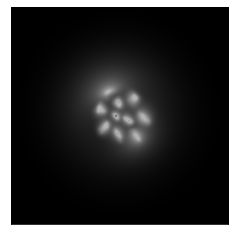
\includegraphics[width=0.8 \textwidth]{sections/006_neurips2020/figures/2D_latent_ours_bn_1.png}
        \caption{Uncertainty - \PostNetacro}
        \label{ours_visualization_unc}
    \end{subfigure}%
    \caption{PriorNet has a pre-ultimate layer of dimension $2$ and was trained with Reverse KL and uniform noise on $[0,255]^{28\times28}$ as OOD data. \PostNetacro has a latent space of dimension $2$ and was trained without OOD data. (a) and (c) show the learned latent positions of data with colored labels. (b) and (d) show uncertainty estimates in the latent spaces where darker regions indicate high uncertainty. \PostNetacro correctly assigns high uncertainty to OOD regions contrary to PriorNet.}
    \label{fig:mnist_2D_latent_space}
	% \vspace{-.5cm}
\end{figure}

% \paragraph{Related work.} Uncertainty estimation is a growing research area unifying various approaches \cite{bayesian-networks, simple-baseline-uncertainty, practical_deep_bayesian_principles, Eswaran2017, ensembles, dropout}. Bayesian Neural Networks learn a \emph{distribution} over the weights \cite{bayesian-networks, simple-baseline-uncertainty, practical_deep_bayesian_principles}. Another class of approaches uses a collection of sub-models and aggregates their predictions, which are in turn used to estimate statistics (e.g., mean and variance) of the class probability distribution. Even though such methods, like ensemble and drop-out, have demonstrated remarkable performance (see, e.g., \cite{dataset-shift}), they describe implicit distributions for predictions and require a costly sampling phase at inference time for uncertainty estimation. 

Recently, a new class of evidential models aim to directly predict the parameters of a prior distribution on the categorical probability predictions, accounting for the different types of uncertainty \cite{PriorNetworks, reverse-kl, sensoy2018, uceloss}. However, these methods require (i) the definition of arbitrary target prior distributions \cite{PriorNetworks, reverse-kl, sensoy2018}, and most importantly, (ii) out-of-distribution (OOD) samples during training time, which is an unrealistic assumption in most applications \cite{PriorNetworks, reverse-kl}.

Classically, these models would use both ID and OOD samples (e.g. MNIST and FashionMNIST) during training to detect similar OOD samples (i.e. FashionMNIST) at inference time. We show that preventing access to explicit OOD data during training leads to poor results using these approaches (see \cref{fig:mnist_2D_latent_space} for MNIST; or \cref{sec:app_additional_results} for toy datasets). Contrary to the expected results, these models produce increasingly confident predictions for samples far from observed data. 

\paragraph{Contributions.} In contrast, we propose  in this chapter, \PostNet (\PostNetacro), which assigns high epistemic uncertainty to out-of-distribution samples, low overall uncertainty to regions nearby observed data of a single class, and high aleatoric and low epistemic uncertainty to regions nearby observed data of different classes. \PostNetacro uses normalizing flows to learn a distribution over Dirichlet parameters in latent space. We enforce the densities of the individual classes to integrate to the number of training samples in that class, which matches well with the intuition of Dirichlet parameters corresponding to the number of observations per class. \PostNetacro does not require any OOD samples for training, the (arbitrary) specification of target prior distributions, or costly sampling for uncertainty estimation at test time.
